\documentclass{article}[12 pt]
\usepackage{amssymb}
\usepackage{amsthm}
\usepackage{amsmath}
\usepackage{appendix}
\usepackage{array}
\usepackage{geometry}
\usepackage{enumitem}
\usepackage{graphicx}
\usepackage{subfig}
\usepackage{caption}
\usepackage{url}
\usepackage{float}
\usepackage{pdfpages}
\usepackage{shortvrb}
\usepackage{mathtools}
\usepackage{multirow}
\usepackage{hyperref}
\usepackage{commath}
\usepackage{bm}
\usepackage{tabularx}


\def\BibTeX{{\rm B\kern-.05em{\sc i\kern-.025em b}\kern-.08em
		T\kern-.1667em\lower.7ex\hbox{E}\kern-.125emX}}


\graphicspath{{"/media/edrive/Bayesian_Methods/BHM_Assignments/HW02/Report/Images/"}}
\geometry{margin=1 in}

\newcommand{\smallvskip}{\vspace{5 pt}}
\newcommand{\medvskip}{\vspace{30 pt}}
\newcommand{\bigvskip}{\vspace{100 pt}}
\newcommand{\tR}{\mathtt{R}}




\begin{document}
	
\begin{center}
	\textbf{\Large Connor McCurley} \\
	AGR 6932  \qquad \quad \quad \textbf{\large Homework 2} \quad \quad \qquad Fall 2019 
\end{center}


%===================================================
%=================== Question 1 ====================
%===================================================

\section*{Question 1}
A \textit{probability mass function} operates on discrete random variables.  Its evaluation returns the probability that a random variable will take on the value of its argument.  A \textit{probability  density function}, on the other hand, operates over continuous random variables.  Probability density functions do not return probability values, but probability densities. Integration must be applied to return the probability over an interval. \\

\noindent
As stated in the class textbook, a \textit{random variable} is a quantity that can take on values due to chance.  They do not have a single value, but instead can take on a range of values.  The important distinction between random variables and the parameters of a probability distribution is that random variables are governed by probability distributions (and hence the parameters of the distributions).  In some cases, the parameters of a distribution can also be modeled as random variables. 


%===================================================
%=================== Question 2 ====================
%===================================================
\section*{Question 2}
The following plots demonstrate convergence of the Binomial and Poisson distributions to a Normal.  It can be observed in Figure \ref{fig:q2_pois_to_normal}, that as the $\lambda$ parameter of the Poisson grows to infinity, the distribution of samples converges to a Normal centered at $\lambda$.  The same is true for the Binomial in Figure \ref{fig:q2_bin_to_normal}.  For a fixed probability of success, $p=0.5$, the distribution converges to a Normal. 

\begin{figure}[H]%
	\centering
	\subfloat[$\lambda=1$]{{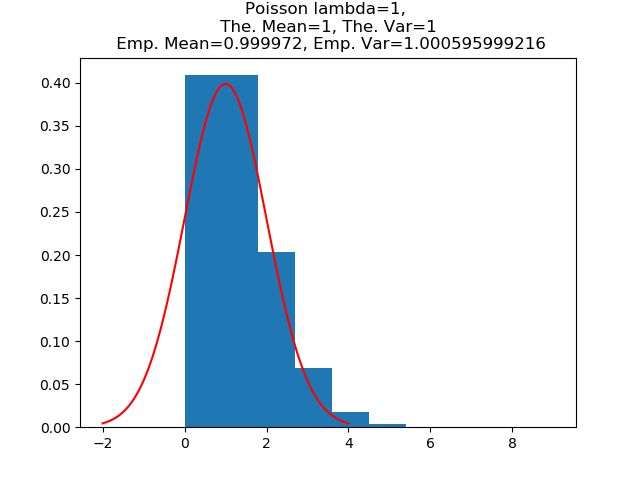
\includegraphics[width=5cm]{q2_pois_1} }}%
	\qquad
	\subfloat[$\lambda=10$]{{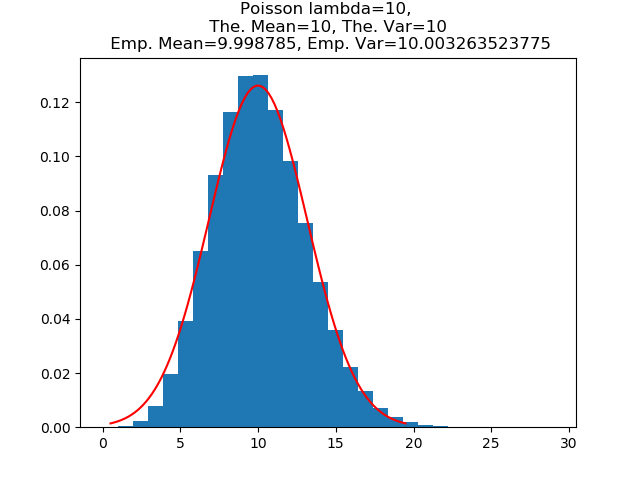
\includegraphics[width=5cm]{q2_pois_10} }}%
	\qquad
	\subfloat[$\lambda=100$]{{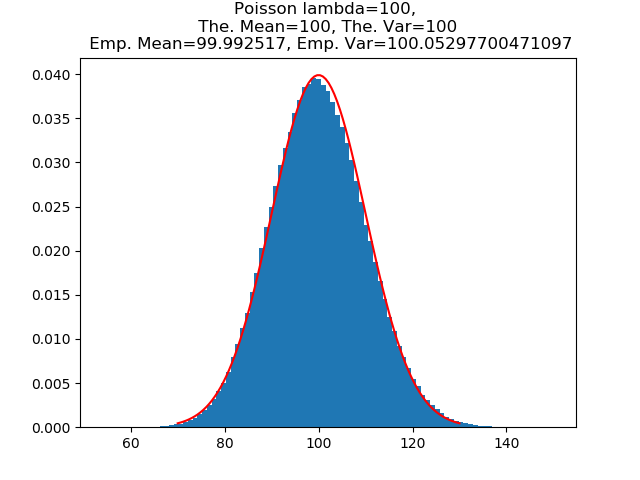
\includegraphics[width=5cm]{q2_pois_100} }}%
	\qquad
	\subfloat[$\lambda=1000$]{{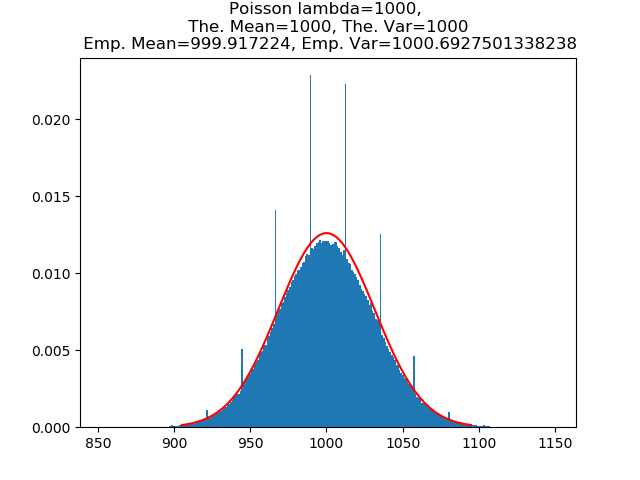
\includegraphics[width=5cm]{q2_pois_1000} }}%
	\caption{Convergence of the Poisson distribution to a Normal distribution for a fixed number of samples, $n=100000$. As the mean parameter $\lambda$ goes to infinity, the distribution of Poisson samples converges to a Normal.}%
	\label{fig:q2_pois_to_normal}%
\end{figure}

\begin{figure}[H]%
	\centering
	\subfloat[$n=10$]{{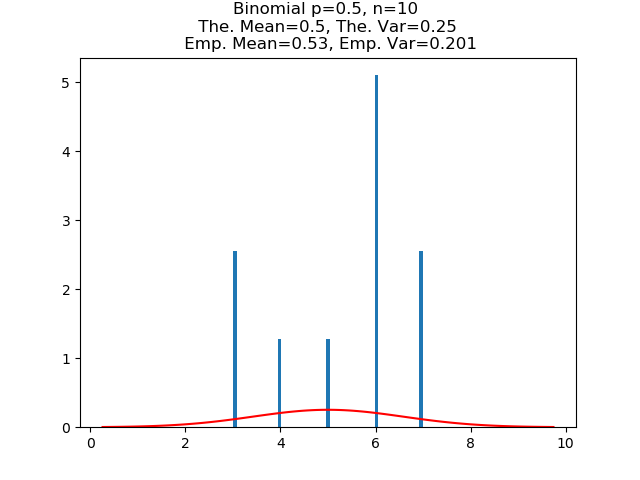
\includegraphics[width=5cm]{q2_bin_10} }}%
	\qquad
	\subfloat[$n=100$]{{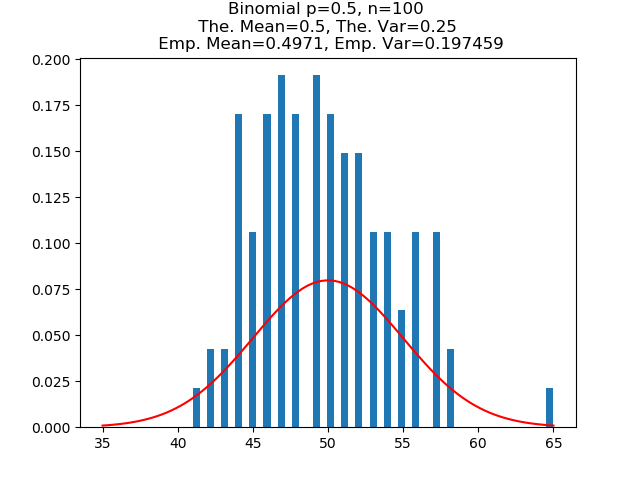
\includegraphics[width=5cm]{q2_bin_100} }}%
	\qquad
	\subfloat[$n=1000$]{{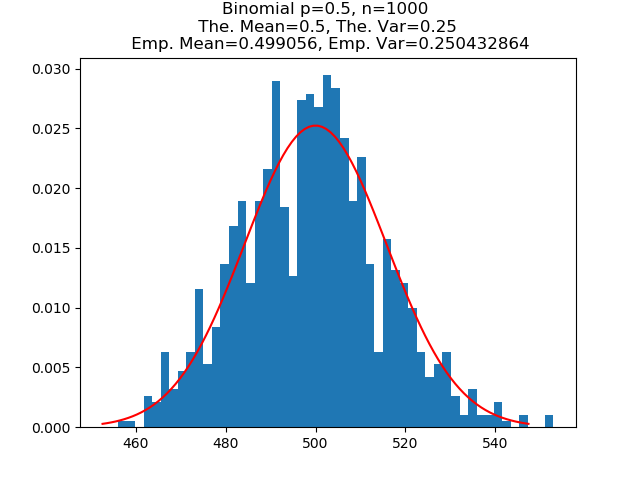
\includegraphics[width=5cm]{q2_bin_1000} }}%
	\qquad
	\subfloat[$n=10000$]{{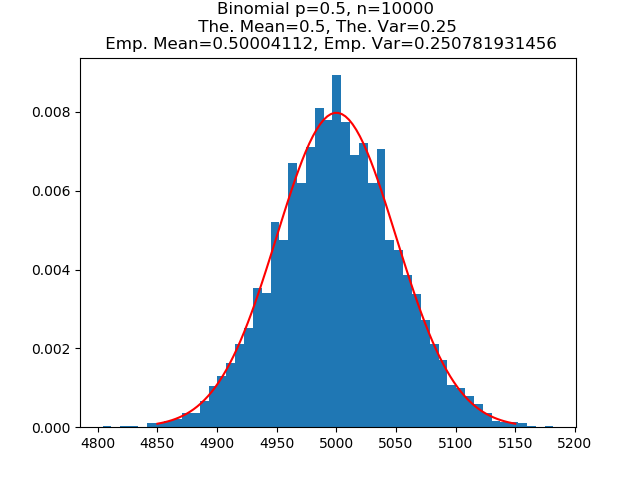
\includegraphics[width=5cm]{q2_bin_10000} }}%
	\qquad
	\subfloat[$n=100000$]{{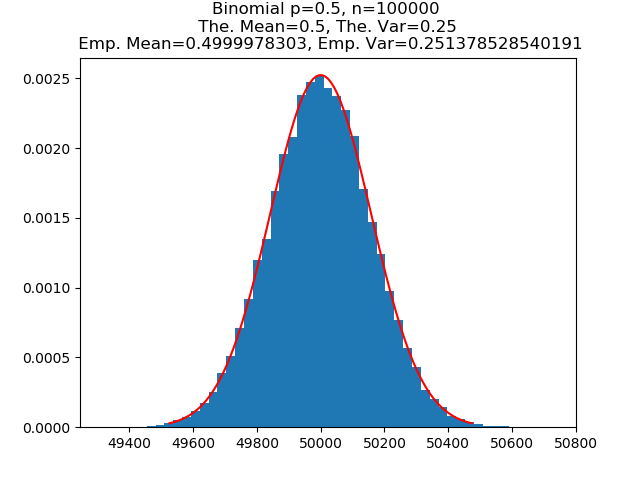
\includegraphics[width=5cm]{q2_bin_100000} }}%
	\qquad
	\subfloat[$n=1000000$]{{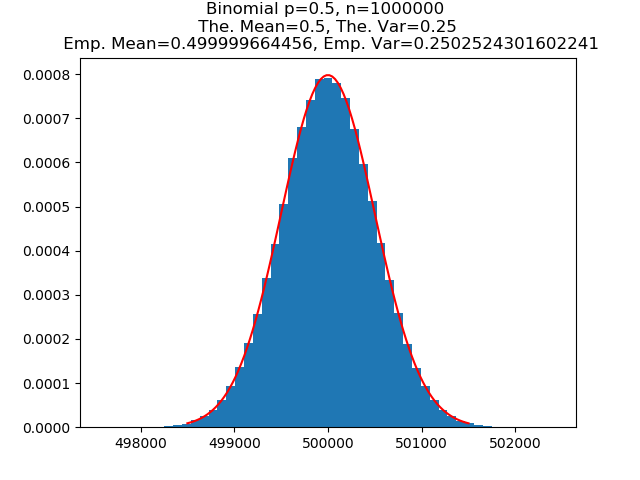
\includegraphics[width=5cm]{q2_bin_1000000} }}%
	\caption{Convergence of the Binomial distribution to a Normal distribution.  The true $p$ value of the Binomial was fixed at $p=0.5$.  As N goes to infinity, the distribution of Binomial samples converges to a Normal.}%
	\label{fig:q2_bin_to_normal}%
\end{figure}



%===================================================
%=================== Question 3 ====================
%===================================================
\newpage
\section*{Question 3}

For the Gamma distribution, gamma($\alpha$,$\beta$), it is known that the skewness is parameterized by the shape, or $\gamma=\frac{2}{\sqrt{\alpha}}$.  The class text book used moment matching with the Gamma to find the mean and variance as $\mu=\frac{\alpha}{\beta}$ and $\sigma^2=\frac{\alpha}{\beta^2}$, respectively.  Using moment matching, we can find the skewness as $\gamma=\frac{\mu_3}{(\sigma^2)^{\frac{3}{2}}}$, where $\mu_3 = \mathbb{E}[(X-\mu)^3]=\mathbb{E}[X^3]-3\mu \sigma^2 - \mu^3$ and $ \mathbb{E}[X^3]=\frac{(\alpha+2)(\alpha+1)\alpha}{\beta}$.  Therefore, 
\begin{align*}
	\gamma &= \frac{\mu_3}{(\sigma^2)^{\frac{3}{2}}} \\
	&= \frac{\mathbb{E}[X^3]-3\mu \sigma^2 - \mu^3}{(\sigma^2)^{\frac{3}{2}}} \\
	&= \frac{\frac{(\alpha+2)(\alpha+1)\alpha}{\beta} - 3(\frac{\alpha}{\beta})(\frac{\alpha}{\beta^2}) - (\frac{\alpha}{\beta})^3}{(\frac{\alpha}{\beta^2})^{\frac{3}{2}}} \\
	&= \frac{2}{\sqrt{\alpha}}
\end{align*}


Figure \ref{fig:q3_gamma_skew} demonstrates pdfs of the Gamma distribution for various shape parameters, $\alpha$.
\begin{center}
	\begin{figure}[H]
		\centering
		\includegraphics[width=0.6\textwidth]{"q3_gamma_skew"}
		\caption{Gamma pdf for various shape parameters, $\alpha$. }
		\label{fig:q3_gamma_skew}
	\end{figure}
\end{center}


%===================================================
%=================== Question 4 ====================
%===================================================
\section*{Question 4}
Binomial sampling experiments were repeated $10^5$ times for the parameterizations requested in the assignment handout.  The standard errors for were computed for each trial.  The results are shown in Table \ref{tab:q4_standard_error}.  As can be observed, the deviation of the error decreases as the number of flips increases.

\begin{table}[H]
	\caption{Standard deviation of the point error for the proportion of heads from Binomial samples.}
	\label{tab:q4_standard_error}
	\begin{center}
		\begin{tabularx}{\textwidth}{ |X|X|X|X|X| } 
			\hline
			\textbf{Number of Flips} & 5 & 10 & 50 & 100\\
			\hline
			\textbf{Standard Error} & 0.205 & 0.145 & 0.065 & 0.046 \\
			\hline
		\end{tabularx}
	\end{center}
\end{table}


\noindent
Manipulating the Chebychev inequality, we can place bounds on the expected value of the proportion of heads.  The Chebychev inequality states that for a random variable $X$ whose governing distribution has mean $\mu$, that

\begin{align*}
	P\{|X-\mu| \geq d\} \leq \frac{\sigma^2}{d^2}
\end{align*}

\noindent
Then for the standard error of the estimate for $p$, denoted as $\bar{p}$:

\begin{align*}
	P \left \{|\bar{p}-p| \leq 2 \frac{\sigma}{\sqrt{N}} \right \}\approxeq 0.95
\end{align*}


%===================================================
%=================== Question 5 ====================
%===================================================
\section*{Question 5}

The maximum likelihood estimator for the $p$ value of a Binomial was found as:
\begin{align*}
	\hat{p} = \frac{\sum^{N}_{i=1}y_i}{Nn}
\end{align*}

\noindent
The derivation is as follows:

\begin{align*}
	[Y|n,p] &= \prod_{i=1}^{N}{n \choose y_i}p^{y_i}(1-p)^{(n-y_i)} \\
	\Rightarrow \log [Y|n,p] &= \log \prod_{i=1}^{N}{n \choose y_i}p^{y_i}(1-p)^{(n-y_i)} \\
	&= \sum_{i=1}^{N}\left [ \log {n \choose y_i} + y_{i}\log p +(n-y_{i})\log (1-p) \right ] \\
	&= \sum_{i=1}^{N} \log {n \choose y_i} + \log p \sum_{i=1}^{N}y_{i} + \log (1-p) \sum_{i=1}^{N}(n-y_{i}) 
\end{align*}

\noindent
and 

\begin{align*}
\frac{\partial}{\partial p}[Y|n,p] &= \frac{\partial}{\partial p} \left [ \sum_{i=1}^{N} \log {n \choose y_i} + \log p \sum_{i=1}^{N}y_{i} + \log (1-p) \sum_{i=1}^{N}(n-y_{i}) \right ]\\
&= \frac{1}{p}\sum_{i=1}^{N}y_{i} - \frac{1}{1-p} \sum_{i=1}^{N} (n-y_{i})
\end{align*}

\noindent
Equating to zero provides

\begin{align*}
&\frac{1}{p}\sum_{i=1}^{N}y_{i} - \frac{1}{1-p} \sum_{i=1}^{N} (n-y_{i}) = 0\\
&\Rightarrow (1-p)\sum_{i=1}^{N} y_{i} = p \sum_{i=1}^{N}(n-y_{i}) \\
&\Rightarrow p = \frac{\sum_{i=1}^{N} y_{i}}{\sum_{i=1}^{N} n} = \frac{\sum_{i=1}^{N} y_{i}}{Nn}
\end{align*}


\noindent
The maximum likelihood estimator was applied to each of the datasets for $p$.  Figure \ref{fig:q5_mle} demonstrates the histograms of the samples for repeated draws from Binomials.  The MLE estimates for $p$ as well as the number of flips in each Binomial trial are shown in the titles.

\begin{figure}[H]%
	\centering
	\subfloat[Number of Flips = 5]{{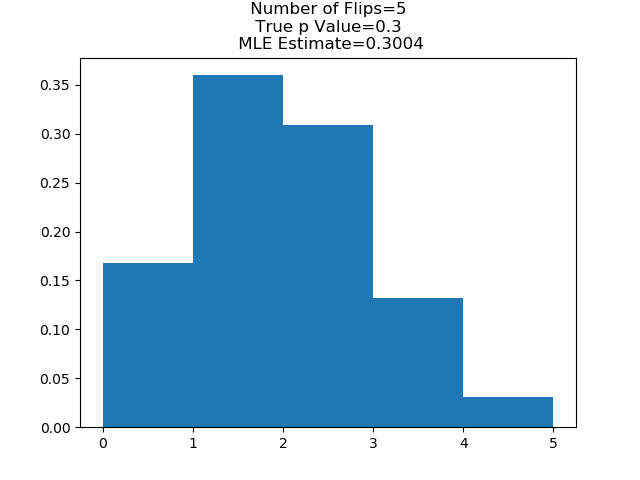
\includegraphics[width=5cm]{q5_mle_5} }}%
	\qquad
	\subfloat[Number of Flips = 10]{{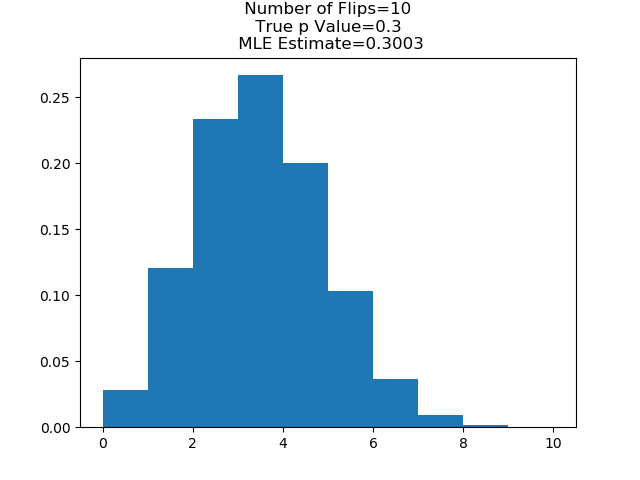
\includegraphics[width=5cm]{q5_mle_10} }}%
	\qquad
	\subfloat[Number of Flips = 50]{{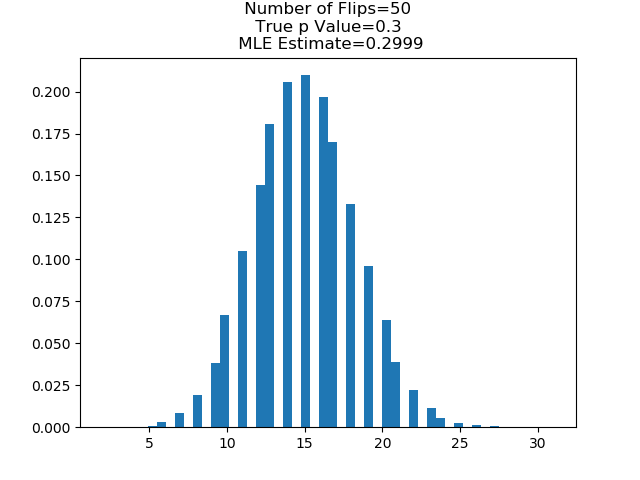
\includegraphics[width=5cm]{q5_mle_50} }}%
	\qquad
	\subfloat[Number of Flips = 100]{{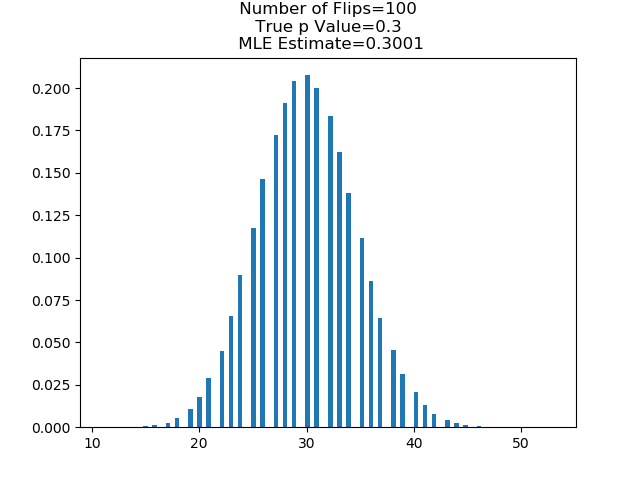
\includegraphics[width=5cm]{q5_mle_100} }}%
	\caption{Histograms of samples drawn from Binomial distributions parameterized by various numbers of flips.}%
	\label{fig:q5_mle}%
\end{figure}

\noindent
Figure \ref{fig:q5_mle} demonstrates the standard errors from 100 Monte Carlo simulations for various parameterizations of the Binomial distribution.  As seen in the figure, the standard deviation of the parameter estimate error decreases as the number of flips increases.  

\begin{figure}[H]%
	\centering
	\subfloat[Number of Flips = 5]{{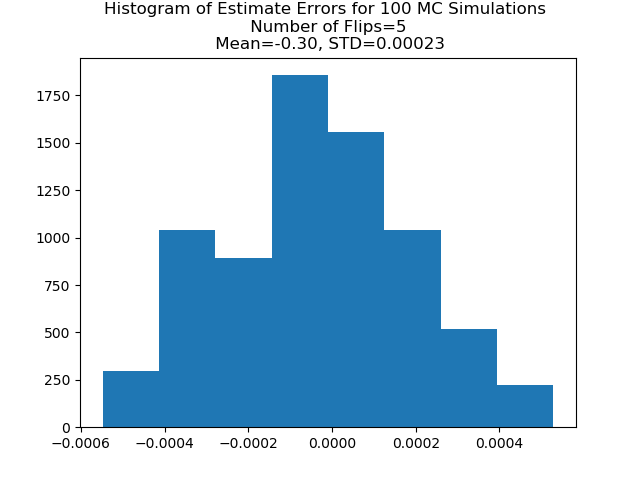
\includegraphics[width=5cm]{q5_mc_5} }}%
	\qquad
	\subfloat[Number of Flips = 10]{{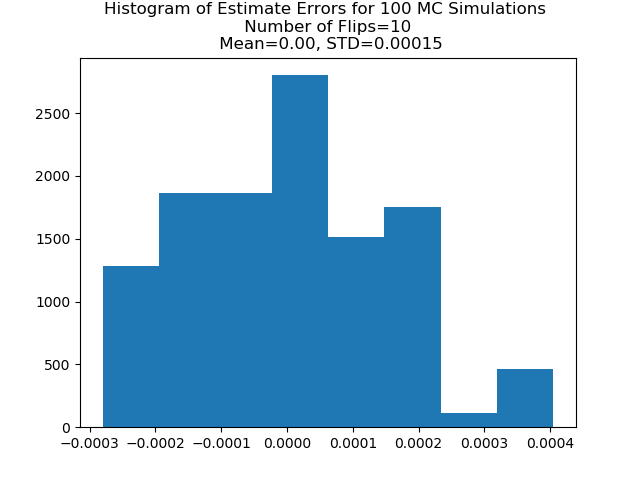
\includegraphics[width=5cm]{q5_mc_10} }}%
	\qquad
	\subfloat[Number of Flips = 50]{{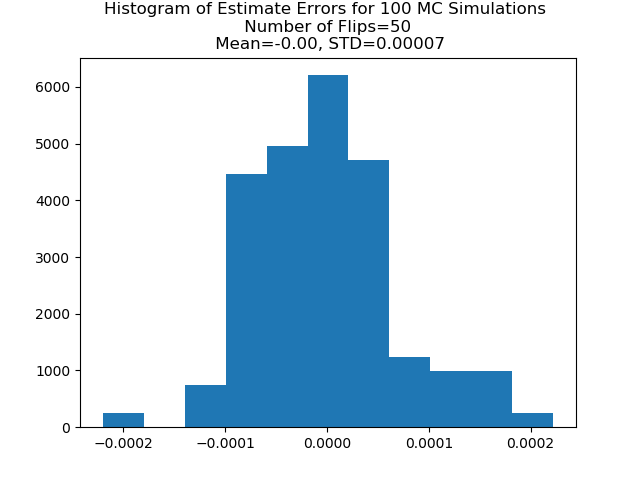
\includegraphics[width=5cm]{q5_mc_50} }}%
	\qquad
	\subfloat[Number of Flips = 100]{{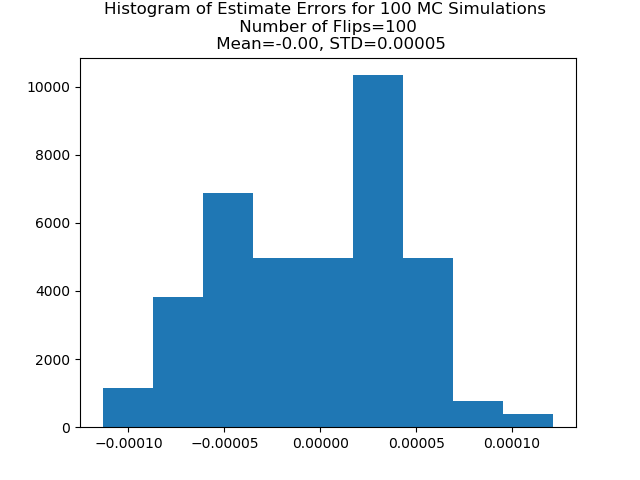
\includegraphics[width=5cm]{q5_mc_100} }}%
	\caption{Histograms of the parameter estimate error for $p$. Each histogram represents the estimate errors }%
	\label{fig:q5_mc}%
\end{figure}


%===================================================
%=================== Question 6 ====================
%===================================================
\section*{Question 6}

Question 6 provided us the differential equation:

\begin{align*}
	\frac{dN}{dt} = rN(1-\frac{N}{K})
\end{align*}

\noindent
By observation, $\lim_{N\to\infty} \frac{dN}{dt} = - \infty$.  The function attains its maximum value at an inflection point, found as 

\begin{align*}
	\frac{\partial}{\partial N} \frac{dN}{dt} &= \frac{\partial}{\partial N} rN - \frac{rN^2}{K} \\
	&= r -\frac{2rN}{K} \\
	&= 0 \\
	& \Rightarrow N = \frac{K}{2}
\end{align*}

\noindent
This is reinforced by Figure \ref{fig:q6_trajectories}, which shows trajectories of $\frac{dN}{dt}$ for various values of $r$ and $K$.

\begin{center}
	\begin{figure}[h]
		\centering
		\includegraphics[width=0.75\textwidth]{"q6_trajectories"}
		\caption{Trajectories of $\frac{dN}{dt}$ for various values of $r$ and $K$.  Each trajectory attain its maximum at $N=\frac{K}{2}$. }
		\label{fig:q6_trajectories}
	\end{figure}
\end{center}

\noindent
The process was then implemented as described in the homework handout.  Figure \ref{fig:q6_observation_error} demonstrates $10^3$ sample paths of the process.  Zero-mean observation error parameterized by a Normal(0, 0.5) was applied to the measurements.   It can be observed that, while the paths showed deviation, they were relatively stable with a consistent mean.

\begin{center}
	\begin{figure}[H]
		\centering
		\includegraphics[width=0.75\textwidth]{"q6_observation_error"}
		\caption{Sample paths of the process $N$ with zero-mean observation error.}
		\label{fig:q6_observation_error}
	\end{figure}
\end{center}

\noindent
The previous trial was repeated with process error instead of observation error.  Figure \ref{fig:q6_process_error} shows the resulting $10^3$ sample paths.

\begin{center}
	\begin{figure}[H]
		\centering
		\includegraphics[width=0.75\textwidth]{"q6_process_error"}
		\caption{ }
		\label{fig:q6_process_error}
	\end{figure}
\end{center}

\noindent
It can be observed that the process error avalanches for specific sample paths, thus forcing the trajectories to $-\infty$.


\end{document}
